\subsection{Obiettivi del prodotto}
	L'obiettivo del prodotto è quello di fornire agli utenti una piattaforma online in cui sia possibile trovare, creare e svolgere esercizi di analisi grammaticale, con lo scopo di poter formare un correttore automatico raccogliendo e immagazzinando i dati. 
La proponente ha imposto i seguenti vincoli sull'implementazione del prodotto:

\subsubsection{Obbligatori}
\begin{itemize}
	\item l'utente deve poter chiedere al sistema di svolgere automaticamente un esercizio mediante un software basato sull'apprendimento supervisionato;
	\item l'utente deve poter correggere l'output automatico generato dal correttore e di salvare il risultato finale;
	\item l'utente deve poter scaricare i dati collezionati nella piattaforma.
\end{itemize}
\subsubsection{Desiderabili}
\begin{itemize}
	\item l'utente dovrebbe avere la possibilità di personalizzare i dati prima di scaricarli dalla piattaforma;
	\item l'utente dovrebbe avere la possibilità di differenziare tra esercizi pubblici e privati.
\end{itemize}
\subsubsection{Opzionali}
\begin{itemize}
	\item l'utente potrebbe voler salvare l'intera cronologia delle modifiche di alcuni dati;
	\item l'utente potrebbe voler creare e/o scaricare un modello direttamente dalla piattaforma.
\end{itemize}

\subsection{Tipologie di utenti}
Gli utenti sono suddivisibili nelle seguenti categorie: 
\begin{itemize}
	\item \textbf{Moderatore:} si occupa di verificare che le persone rispettino il codice di comportamento della piattaforma e della gestione degli esercizi presenti in essa;
	\item \textbf{Sviluppatore:} è interessato alla consultazione dei dati raccolti, magari applicando filtri o visualizzando lo storico delle annotazioni;
	\item \textbf{Utente generico:} è la tipologia di utente più comune che è interessato alla ricerca e allo svolgimento di esercizi sulla piattaforma.
\end{itemize}

Quest'ultima categoria è suddivisibile ulteriormente in:
\begin{itemize}
	\item \textbf{Utente non riconosciuto:} è l'utente che non ha il pieno accesso alle funzionalità dell'applicazione.
	\item \textbf{Utente riconosciuto:} è l'utente che ha le credenziali e ha effettuato l'accesso.
\end{itemize}

L'utente riconosciuto individua due sottocategorie:
\begin{itemize}
	\item \textbf{Allievo:} gli allievi possono iscriversi alle classi, gestire tali iscrizioni e visualizzarne i dati.
	\item \textbf{Insegnante:} gli insegnanti possono inserire soluzioni degli esercizi, gestire le proprie classi e visualizzare il rendimento dei propri alunni.
\end{itemize}
\begin{figure}[h]
			\centering
			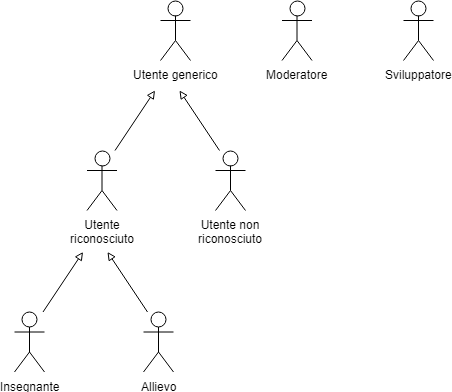
\includegraphics[scale=0.7]{images/attori.png}
			\caption{Attori del progetto}
		\end{figure}
		
\subsection{Funzionalità del prodotto}
	\subsubsection{Funzionalità per l'utente generico}
	Il prodotto offre la possibilità a tutti gli utenti di svolgere esercizi sull'analisi grammaticale e ottenere velocemente una soluzione. Per far ciò è necessario che l'utente possa o inserire una frase o cercarne una all'interno della piattaforma, tramite una vista di inserimento (la pagina principale) nel primo caso e una di ricerca nel secondo. In seguito, dopo aver raggiunto una schermata contenente la frase suddivisa in parole, l'utente deve poter inserire la propria soluzione. Infine, verrà visualizzata una schermata con la valutazione dell'esercizio.
	La ricerca deve poter essere raffinata in base agli autori, la difficoltà e agli argomenti degli esercizi.
	\paragraph{Funzionalità per l'utente riconosciuto\\}
	L'utente riconosciuto può accedere a una schermata con le informazioni del proprio profilo e all'occorrenza modificarlo. \`E infine disponibile la funzionalità di logout. In base al tipo di utente riconosciuto cambiano le altre funzionalità disponibili.
	\subparagraph{Funzionalità per l'insegnante\\}
	L'insegnante può inserire esercizi tramite una schermata di inserimento, modificare gli esercizi inseriti. Inoltre, per quest'utente deve essere possibile gestire le proprie classi. Segue che la piattaforma deve rendere disponibili le funzionalità di creazione ed eliminazione di una classe. Per le varie classi, l'insegnante può inserire (o eliminare) gli alunni, assegnare gli esercizi e visualizzare l'andamento dei propri alunni.
	\subparagraph{Funzionalità per l'allievo\\}
	L'allievo può visualizzare i propri progressi (magari tramite grafici) che mostrano il proprio andamento nelle valutazioni in modo da capire come prosegue il proprio apprendimento. Inoltre, l'allievo può vedere la lista delle classi a cui è iscritto e ottenere le informazioni riguardanti tali classi, come ad esempio la media degli alunni, il numero degli allievi iscritti e gli esercizi assegnati.
	\paragraph{Funzionalità per l'utente non riconosciuto\\}
	L'utente non riconosciuto dal sistema può visualizzare una schermata di registrazione o una pagina di autenticazione. Nella prima, è possibile registrarsi come allievo o insegnante, nella seconda è possibile effettuare l'accesso alla piattaforma tramite le proprie credenziali.
	
	\subsubsection{Funzionalità per il moderatore}
	Il moderatore avrà un accesso privilegiato alla piattaforma tramite una vista differente dagli altri utenti, in cui sarà immediatamente visibile la lista degli utenti che hanno richiesto la registrazione come insegnante. Deve essere possibile per il moderatore effettuare la verifica di tali richieste. Inoltre, il moderatore deve poter eliminare gli esercizi e gli utenti visualizzare la lista delle segnalazioni.
	
	\subsubsection{Funzionalità per lo sviluppatore}
	Lo sviluppatore avrà un accesso privilegiato alla piattaforma tramite una vista differente dagli altri utenti, in cui sarà immediatamente visibile la ricerca delle annotazioni inserite nella piattaforma. La ricerca deve poter essere raffinata in base al tempo di inserimento e in base agli autori delle annotazioni. Per ogni annotazione deve poterne consultare i dati. Deve, inoltre, essere disponibile la visualizzazione dello storico delle annotazioni inserite. Lo sviluppatore può scaricare i dati raccolti e il dataset risultante in base a una ricerca effettuata. Infine, deve essere possibile per quest'utente il download di un modello, la creazione di uno nuovo o il cambio del modello usato dalla piattaforma.